\documentclass[a4paper, titlepage]{jsarticle}

\usepackage[utf8]{inputenc}

\usepackage[dvipdfmx]{graphicx}
\usepackage[dvipdfmx]{xcolor}

\usepackage{hyperref}
\usepackage{mathtools}
\usepackage{tikz}
\usepackage{amsmath}
\usepackage{amssymb}
\usepackage{amsfonts}
\usepackage{latexsym}
\usepackage{enumitem}
\usepackage{empheq}
\usepackage{amsthm}
\usepackage{bm}
\usepackage{physics}

\usetikzlibrary{
   positioning,
   arrows.meta,
   graphs
}

\title{\Huge 予測符号化とbPCモデルについて}
\author{\Large 創域理工学部\quad 情報計算科学科\quad 4年\\\Large 学籍番号\;:\;6322045\\\Large 砂川恵太朗}
\date{\today}

\begin{document}

\maketitle

\section{予測符号化について}
以下のサブセクションは,論文"PREDICTIVE CODING: A THEORETICAL AND EXPERIMENTAL REVIEW"に基づいている.
\subsection{予測符号化の大まかな概要}
\begin{itemize}
   \item 根幹となる働きは,予測した入力と実際に受け取った入力の差である「予測誤差」を最小化すること
   \item 予測誤差の最小化には,知覚にあたる隠れ状態の即時推論や,学習にあたるグローバルな世界モデルの更新,立てた予測に合致するような入力を外界からサンプリングするなどして行う
   \item 感覚入力に含まれるノイズの度合いによって,その感覚入力の信頼性を評価し,ノイズが少ない入力に対して注意を払ういわゆる「アテンション」に近い動作をとる
   \item 脳は階層構造をとっているという前提の下,予測誤差はモデル全体ではなく各層の間でへブ学習則に従ってローカルに計算される
   \item 知覚的推論と学習は,早い時間スケールでのニューロン発火率(単位時間当たりにどれだけ発火するか)の最適化と,遅い時間スケールでのシナプスの重みの最適化で予測誤差を最小化することで実行可能であるという
\end{itemize}

\subsection{予測符号化の数学的成り立ち}
\subsubsection{変分推論としての予測符号化}
変分推論とは,統計物理学における扱いにくい最適化問題を近似的に解く手法から発展したもので,直観的には,近似的な変分密度を仮定し,その統計量を最適化した後それを望ましい推論分布に一致させようとする方法である.
\par
数学的に形式化するために,観測データ$o$があって潜在状態$x$を推定したいとする.そして生成モデルとして\;$p(o,x)=p(o|x)p(x)$\;を仮定する.ベイズの定理により\;$\displaystyle\frac{p(o,x)}{p(o)}=p(x|o)$\;とすることで真の事後分布$p(x|o)$を直接計算できるが,正規化因子(事後確率を正規化する定数)\;$p(o)=\int dxp(o,x)$\;はすべての潜在状態について計算する必要があるため計算困難になることがしばしばある.周辺尤度$p(o)$は生成モデルパラメータの取りうる値について平均化された,与えられたモデルにおけるデータの尤度を効果的に評価するため,しばしばエビデンスと呼ばれる.周辺尤度$p(o)$の計算は,ベイズモデル比較法において中核的な量であり,2つの異なる生成モデルがデータに適合する能力を比較するために用いられるため,本質的に価値がある.
\par
真の事後分布$p(x|o)$をベイズ規則によって直接計算することは一般的に困難であるため,変分推論ではパラメータ$\phi$をもつ補助的な事後分布$q(x|o;\phi)$を用いて真の事後分布を近似することを目指す.この変分$q$分布は任意であり,エージェントの制御下にある.目標は,この近似事後分布と真の事後分布との間の発散をパラメータに関して最小化することで,近似事後分布を真の事後分布に適合させることである.数学的には,この問題は以下のように記述できる.
\begin{equation}
   q^*(x|o;\phi)=\underset{\phi}{argmin}\;\mathbb{D}[q(x|o;\phi)||p(x|o)]
\end{equation}
$\mathbb{D}[\cdot]$はカルバック・ライブラー情報量で,異なる2つの分布間の距離に相当するものを計算する(厳密には距離ではない).このように事後分布の計算という推論問題を,カルバック・ライブラー情報量を最小化する最適化問題に置き換えることができる.しかし,この方法で問題を記述しても,最適化する必要がある発散が依然として計算不能な真の事後分布を含んでいるため,最適化は達成されない.したがって,代わりにこの量の上界である変分自由エネルギーと呼ばれる計算可能な量を最適化することで代替する.この上界を生成するために,単純にベイズの規則を真の事後分布に適用し,生成モデルとエビデンスの形式に書き換える.
\begin{equation}
   \begin{aligned}
      D_{\mathrm{KL}}[q(x|o;\phi)||p(x|o)]&=D_{\mathrm{KL}}\qty[q(x|o;\phi)||\frac{p(o,x)}{p(o)}] \\
      &=D_{\mathrm{KL}}[q(x|o;\phi)||p(o,x)]+\mathbb{E}_{q(x|o;\phi)}[\ln p(o)] \\
      &=D_{\mathrm{KL}}[q(x|o;\phi)||p(o,x)]+\ln p(o) \\
      &\le D_{\mathrm{KL}}[q(x|o;\phi)||p(o,x)]=\mathcal{F}
   \end{aligned}
\end{equation}
変分自由エネルギー$\mathcal{F} = D_{\mathrm{KL}}[q(x|o; \phi)||p(o, x)]$は,確率として $0 ≤ p(o) ≤ 1$より$\ln p(o)$ は必然的に 0以下 となるため,上限になる.重要なのは,$\mathcal{F}$ が扱いやすい量であるということである.これは,モデル作成者として私たちが知っていると仮定する2つの量,すなわち変分近似事後分布 $q(x|o)$ と生成モデル $p(o, x)$ の間の乖離である.$\mathcal{F}$は上限であるため,$\mathcal{F}$を最小化することで,$q(x|o; \phi)$ を真の事後分布に近づけることができる.さらに,$q(x|o; \phi) = p(x|o)$ の場合には $\mathcal{F} = \ln p(o)$ ,つまりモデル証拠となり,このような場合には $\mathcal{F}$ をモデル選択に使用できることを意味する.また,変分自由エネルギー$\mathcal{F}$は次のような2つの項に分解することができる.
\begin{equation*}
   \begin{aligned}
      \mathcal{F}&=D_{\mathrm{KL}}[q(x|o;\phi)||p(o,x)] \\
      &=\underbrace{\mathbb{E}_{q(x|o;\phi)}[\ln p(o|x)]}_{\mathrm{Accuracy}}+\underbrace{D_{\mathrm{KL}}[q(x|o;\phi)||p(x)]}_{\mathrm{Complexity}}
   \end{aligned}
\end{equation*}
Accuracy項は観測データが生成モデルに対して尤もらしいかを示す尤度項で,Complexity項は事前分布から近似事後分布がどれだけ異なっているかを示していて,$\mathcal{F}$の最小化にはAccuracy項を最大化させ,Complexity項を最小化させる.これよりAccuracy項は尤度最大化項ともいう.
\par
多くの場合,生成モデル$p(o,x)$を知っているという仮定を緩和して,生成モデルの具体なパラメータが既知であるという前提を放棄する必要がある.幸い,この緩和は致命的にはならない.仮定を緩和する代わりに,期待値最大化(EM)アルゴリズムを用いて,生成モデルと変分事後分布を同時に学習することが必要になる.EMアルゴリズムは非常に直感的である.まず,未知の生成モデルをパラメータ $\theta$でパラメータ化し,これを任意の初期値 $\theta_0$で初期化する.同様に,変分事後分布も任意の初期値$\phi_0$で初期化する.次に,変分事後分布のパラメータ $\phi$について$\mathcal{F}$を最適化し(生成モデルのパラメータ$\theta$は固定),その後,逆に生成モデルのパラメータ$\theta$について$\mathcal{F}$を最適化する(変分事後分布のパラメータ$\phi$は固定)という交互最適化を行う.数学的には,この交互最適化は以下のように記述される.
\begin{equation}
   \begin{aligned}
      \phi_{t+1}&=\underset{\phi}{argmin}\mathcal{F}(\phi,\theta)|_{\theta=\theta_t} \\
      \theta_{t+1}&=\underset{\theta}{argmin}\mathcal{F}(\phi,\theta)|_{\phi=\phi_{t+1}}
   \end{aligned}
\end{equation}
変分推論の一般原理を確認したところ,これらが予測符号化とどのように関連しているかが判明した.まず,具体的な変分推論アルゴリズムを得るためには,変分事後分布と生成モデルの形式を指定する必要があります.予測符号化を得るために,生成モデルにガウス形式\;$p(o,x;\theta)=p(o|x;\theta)p(x;\theta)=\mathcal{N}(o;f(\theta_1x),\Sigma_1)\mathcal{N}(x;g(\theta_2\bar{\mu}),\Sigma_2)$\;を仮定する.尤度ガウス分布の平均は,パラメータ$\theta$でパラメータ化された隠れ状態$x$の関数$f$と仮定し,事前ガウス分布の平均は,事前平均$\bar{\mu}$の任意関数$g$に設定される.生成モデルの2つのガウス分布の分散は$\Sigma_1$と$\Sigma_2$で表される.また,変分事後分布はディラック・デルタ(または点質量)分布 \;$q(x|o;\phi)=\delta(x-\mu)$\;と仮定し,中心は\;$\phi=\mu$\;である.
\par
これらの変分事後分布と生成モデルの定義が与えられると,最適化される変分自由エネルギーの具体的な形式を書き出すことができる.まず,変分自由エネルギーを「エネルギー」項と「エントロピー」項に分解する.
\begin{equation}
   \begin{aligned}
      \mathcal{F}&=D_{\mathrm{KL}}[q(x|o;\phi)||p(o,x;\theta)] \\
      &=\underbrace{\mathbb{E}_{q(x|o;\phi)}[\ln q(x|o;\phi)]}_{\mathrm{Entropy}}-\underbrace{\mathbb{E}_{q(x|o;\phi)}[\ln p(o,x;\theta)]}_{\mathrm{Energy}}
   \end{aligned}
\end{equation}
ここで,ディラック・デルタ分布のエントロピーは0であるため,エントロピー項は無視し,エネルギー項のみを書き出すことに注力する.
\begin{equation}
   \begin{aligned}
      \underbrace{\mathbb{E}_{q(x|o;\phi)}[\ln p(o,x;\theta)]}_{\mathrm{Energy}}&=\mathbb{E}_{\delta(x-\mu)}[\ln(\mathcal{N}(o;f(\theta_1x),\Sigma_1)\mathcal{N}(x;g(\theta_2\bar{\mu}),\Sigma_2))] \\
      &=\ln(\mathcal{N}(o;f(\theta_1x),\Sigma_1)+\ln\mathcal{N}(x;g(\theta_2\bar{\mu}),\Sigma_2)) \\
      &=-\frac{(o-f(\mu,\theta_1))^2}{2\Sigma_1}-\frac{1}{2}\ln2\pi\Sigma_1-\frac{(\mu-g(\bar{\mu},\theta_2))^2}{2\Sigma_2}-\frac{1}{2}\ln2\pi\Sigma_2 \\
      &=-\frac{1}{2}[\Sigma_1^{-1}\epsilon_o^2+\Sigma_2^{-1}\epsilon_x^2+\ln2\pi\Sigma_1+\ln2\pi\Sigma_2]
   \end{aligned}
\end{equation}
ここで,「予測誤差」$\epsilon_o=o-f(\mu,\theta_1)$\;と\;$\epsilon_x=\mu-g(\bar{\mu},\theta_2)$\;を定義する.したがって,エネルギー項,ひいては変分自由エネルギーは,その逆分散で重み付けされた2つの二乗予測誤差項の合計に,いくつかの追加のログ分散項を加えたものに過ぎない.
\par
最後に,予測符号化の更新ルールを導出するために,さらにもう1つの仮定をおく.変分自由エネルギーは勾配降下法によって最適化される,という仮定である.
\begin{equation}
   \frac{d\mu}{dt}=-\frac{\partial\mathcal{F}}{\partial\mu}
\end{equation}
これを踏まえて,変分自由エネルギー$\mathcal{F}$の微分をとることで,すべての関心のある変数$(\mu,\theta_1,\theta_2)$のダイナミクスを導くことができる.更新規則は以下のとおりである.
\begin{align}
   \frac{d\mu}{dt}&=-\frac{\partial\mathcal{F}}{\partial\mu}=\Sigma_1^{-1}\epsilon_o\frac{\partial f}{\partial\mu}\theta^T-\Sigma_2^{-1}\epsilon_x \\
   \frac{d\theta_1}{dt}&=\frac{\partial\mathcal{F}}{\partial\theta_1}=-\Sigma_1^{-1}\epsilon_o\frac{\partial f}{\partial\theta_1}\mu^T \\
   \frac{d\theta_2}{dt}&=\frac{\partial\mathcal{F}}{\partial\theta_2}=-\Sigma_2^{-1}\epsilon_x\frac{\partial g}{\partial\theta_2}\bar{\mu}^T
\end{align}
\subsubsection{階層的予測符号化}
先のセクションでは単一レベルの予測符号化に焦点を当てたが,このセクションでは階層的な予測符号化について触れていく.機械学習と同様に,予測符号化についても任意の深さの階層的ダイナミクスを扱うように拡張することができる.潜在変数$x_1,x_2,\dots,x_L$の複数層を仮定し,生成モデルを以下のように定義することで実現される.
\begin{equation}
   p(x_0\dots x_L)=p(x_L)\prod_{l=0}^{L-1}p(x_l|x_{l+1})
\end{equation}
ここで,\;$p(x_l|x_{l+1})=\mathcal{N}(x_l;f_l(\theta_{l+1},x_{l+1},\Sigma_l))$\;であり,最終層\;$p(x_L)=\mathcal{N}(x_l|\bar{x}_L,\Sigma_L)$\;は任意の事前分布$\bar{x}_L$を持ち,階層の最下部の潜在変数は実際に入力された観測値\;$x_0=o$\;に設定される.同様に,各層に個別の変分事後分布\;$q(x_{1:L}|o)=\prod_{l=1}^L\delta(x_l-\mu_l)$\;を定義すると,次のように変分自由エネルギーは各層での予測誤差の合計として表される.
\begin{equation}\label{another_VFE}
   \mathcal{F}=\sum_{l=1}^L\Sigma_l^{-1}\epsilon_l^2+\ln2\pi\det(\Sigma_l)
\end{equation}
ここで,$\epsilon_l=\mu_l-f_l(\theta_{l+1},\mu_{l+1})$\;である.

\begin{figure}[htbp]
   \centering
   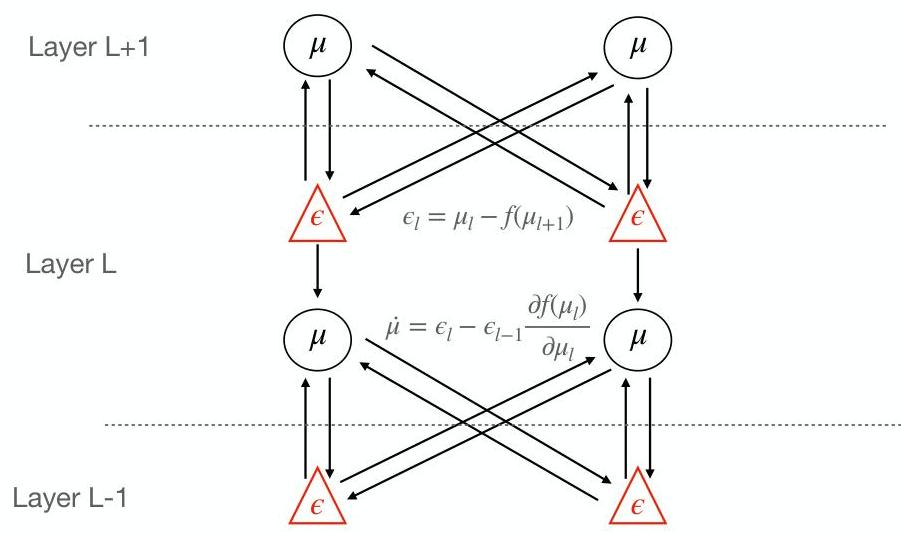
\includegraphics[scale=0.4]{PC_layer.jpeg}
   \caption{
      多層予測符号化ネットワークのアーキテクチャ.価値ニューロン$\mu$は仮想のエラーニューロンと現在の層のエラーニューロンの両方に現在のアクティビティを投影する.エラーニューロンは上層の価値ニューロンからの抑制性トップダウン入力と,現在の層の価値ニューロンからの興奮性入力を受け取る.逆に,価値ニューロンは下層のエラーニューロンから興奮性投影と,現在の層のエラーニューロンから抑制性投影を受け取る.重要なのは,明示的なエラーニューロンを持つこのモデルでは,すべてのシナプス可塑性ルールが純粋にへブ学習則になるということである.
   }
   \label{PC_layer}
\end{figure}

\begin{align}
   \frac{d\mu_l}{dl}&=-\frac{\partial\mathcal{F}}{\partial\mu_l}=\Sigma_{l-1}^{-1}\epsilon_{l-1}\frac{\partial f_{l-1}}{\partial\mu_l}\theta_l^T-\Sigma_l^{-1}\epsilon_l \\
   \frac{d\theta_l}{dl}&=-\frac{\partial\mathcal{F}}{\partial\theta_l}=\Sigma_l^{-1}\epsilon_{l-1}\frac{\partial f_{l-1}}{\partial\theta_l}\mu_l
\end{align}
変分平均 $\mu$ のダイナミクスは,自身の層での予測誤差と下位層からの予測誤差にのみ依存する.直感的には,$\mu$ は上位層からの予測から逸脱することによる誤差の発生と,下位層での誤差を解決するために自身の予測を調整することの間でバランスを取ろうとする.神経学的に実装された階層的予測符号化ネットワークでは,予測誤差のみが感覚データから潜在表現へと「上方」に伝達され,予測は「下方」に伝達される.これは予測符号化の概念を理解する上で重要であり,多くの知覚神経科学モデルで仮定されているように,感覚データが階層を直接伝達されるわけではないことを意味する.$\mu$ のダイナミクスは,生物学的にも妥当性が高いとされている.これは,$\mu$ 自身の層と下位層からの精度重み付けされた予測誤差の合計であるためである.下位層からの予測誤差は,シナプス重み $\theta^T$ を介して活性化関数の勾配 $f_l$ で重み付けされて上方に伝達される.これは,視覚モデルでしばしば仮定されるような直接的な順方向パスが予測符号化には存在しないことを意味する.ただし,順方向パスを追加して予測符号化モデルを拡張することは可能である.重要な点として,シナプス重みのダイナミクスは完全に局所的であり,特定の層における下位層からの予測誤差と現在の $\mu$ のみが必要になる.これにより,ダイナミクスは前シナプス性の $\epsilon_{l-1}$ と後シナプス性の $\mu_l$ の間のヘッブ学習則となり,活性化関数の勾配によって重み付けがなされる.
\subsubsection{予測符号化と精度}
予測符号化フレームワークの角となる側面の1つは,精度または逆分散の概念である.精度は予測誤差の重要性を乗法的に調整する役割を果たし,したがってモデルの全体的なダイナミクスに大きな影響を与える.
\par
数学的には,精度の動的更新則は自由エネルギーの勾配降下法として導出できる.精度は厳密には生成モデルのパラメータであるため,この更新則はEMアルゴリズムにおける追加のM(Maximization)ステップとなる.式\eqref{another_VFE}より,自由エネルギーは次のように書ける.
\begin{equation}
   \mathcal{F}=\sum_{l=1}^L\Sigma_l^{-1}\epsilon_l^2+\ln2\pi\det(\Sigma_l)
\end{equation}
そして精度行列$\Sigma_l^{-1}$のダイナミクスを,分散に関する自由エネルギーの項加法として導くことができる.
\begin{equation}
   \begin{aligned}
      \frac{d\Sigma}{dt}=-\frac{\partial\mathcal{F}}{\partial\Sigma}&=\Sigma_l^{-T}\epsilon_l\epsilon_l^T\Sigma_l^{-T}-\Sigma_l^{-T} \\
      &=\Sigma_l^{-1}\epsilon_l\epsilon_l^T\Sigma_l^{-T}-\Sigma_l^{-1} \\
      &=\bar{\epsilon}_l\bar{\epsilon}_l^T-\Sigma_l^{-1}
   \end{aligned}
\end{equation}
ここで,$\Sigma$は共分散行列であるので,$\Sigma^{-1}=\Sigma^{-T}$\;である.次に,精度重み付け予測誤差を\;$\bar{\epsilon}_l=\Sigma_l^{-1}\epsilon_l$\;として定義した.これらのダイナミクスから,平衡状態にある精度行列は,各層における精度重み付け予測誤差の分散に等しいことがわかる.
\begin{equation}
   \begin{aligned}
      \mathbb{E}\qty[\frac{d\Sigma}{dt}]&=\mathbb{E}[\bar{\epsilon}_l\bar{\epsilon}_l^T]-\Sigma_l \\
      &=\mathbb{E}\qty[\frac{d\Sigma}{dt}]=0\Rightarrow\Sigma_l=\mathbb{E}[\bar{\epsilon}_l\bar{\epsilon}_l^T] \\
      &\Rightarrow\Sigma_l=\mathbb{V}[\bar{\epsilon}]
   \end{aligned}
\end{equation}
実際には,精度ダイナミクスの不動点により,これらの行列は各レベルでの予測誤差の平均分散を単純に表すものになる.階層の最下位レベルでは,予測誤差の分散はデータの固有の分散と強く関連しているため,アルゴリズム的には,学習可能な精度行列によって状態依存の加法ノイズを含むデータの表現と推論が可能になる.様々な知覚システムにおいて,入力される感覚データの変動を表現できることは,そのような感覚ストリームを適切にモデル化し,正確な推論を実行するために非常に重要になる.

\section{Bidirectional predictive coding}
ここからは研究テーマのトピックの1つである Bidirectional predictive coding,bPCモデルについてまとめていく.元論文は"Bidirectional predictive coding"である.
\subsection{導入}
Bidirectional predictive coding モデルでは視覚推論について扱っている.脳がどのように視覚推論を実行するかには,2つの枠組みがある.1つは視覚をボトムアップの識別プロセスとして記述する.これは感覚入力から行動に関連する情報を抽出するプロセスである.もう1つは視覚を生成プロセスとして定式化し,脳が感覚入力のトップダウン予測を生成して,ベイズ推論の結果として脳の内部状態を更新する.視覚推論はこの両方を組み合わせたものである可能性が示唆されているが,その計算モデルのほとんどは識別的か生成敵のどちらかである.両方を組み合わせたモデルは,視覚学習の特徴である教師あり学習または教師なし学習のパフォーマンスのいずれかを妥協しなければならなくなる場合がある.
\par
ここで提案される Bidirectional predictive coding は,予測符号化に基づく生成推論と識別推論の両方を実行できるモデルである.予測符号化は生成推論または識別推論のいずれかとして定式化することができる.また,生成推論または識別推論をサポートするモデルパラメータを学習するためにヘッブ学習則を採用しているため,学習にバックプロパゲーション(BP)に依存するモデルよりも生物学的により妥当性が高い.
\begin{figure}[htbp]
   \centering
   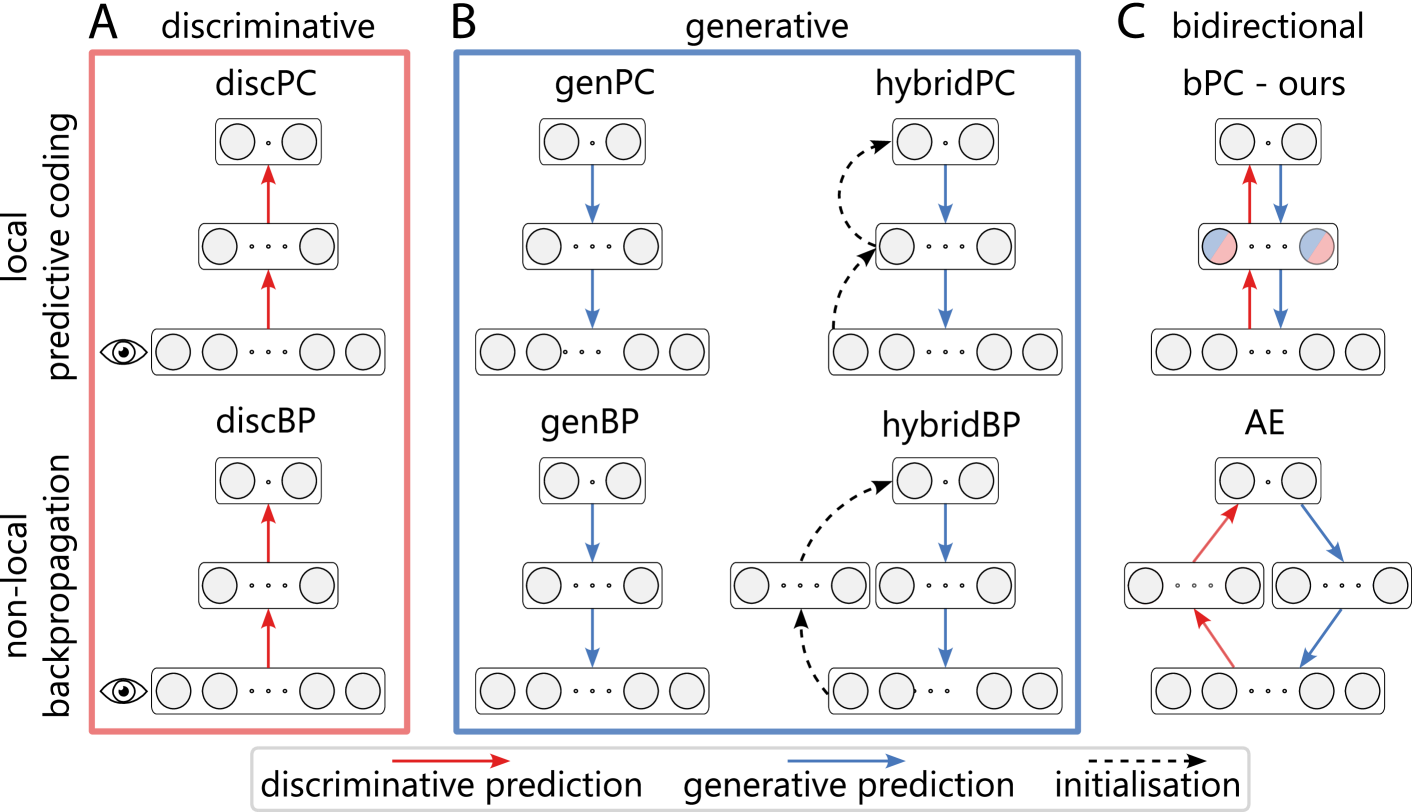
\includegraphics[scale=0.26]{bPC_relatedmodels.png}
   \caption{実験で使用されたモデルアーキテクチャ.矢印は予測の方向を示し,破線矢印は初期化を表す.識別モデル(赤)はボトムアップ予測を行い,生成モデル(青)はトップダウン予測を行い,双方向モデルはその両方を統合する.上段のモデルは局所的な予測符号化計算を実装し,下段のモデルは非局所的なBPベースの計算に依存している.各予測矢印は,ニューラル回路内の双方向接続に対応しており,一方は予測用,もう一方は誤差逆伝播用である.}
   \label{related_models}
\end{figure}
\par
この論文で提案されたことは以下の通りである.
\begin{itemize}
   \item この論文では双方向予測符号化を提案する.これは,単一のエネルギー関数を最小化することから自然に生じる生成推論と識別推論の両方を採用した,生物学的に妥当な視覚知覚モデルである.
   \item bPCは,教師あり分類タスクと教師なし表現学習タスクの両方で,純粋に識別的または生成的な同等のモデルと同様に機能し,先行するハイブリッド予測符号化モデルよりも優れていることを示す.
   \item 我々は,単方向モデルと比較し,分布外データポイントの検出に役立つエネルギーランドスケープ(エネルギー関数の状態)を学習することを示すことにより,両方のタスクでのbPCの優れたパフォーマンスの説明を提供する.
   \item マルチモーダル学習と遮蔽された視覚シーンによる推論を含む2つの生物学的に関連するタスクで bPC が他の PC モデルよりも優れていることを示す.これは,脳内の視覚推論のより忠実なモデルになる可能性を示唆している.
\end{itemize}
\subsection{背景と関連研究}
\begin{enumerate}
   \item \textbf{識別的予測符号化} \\
   近年の研究では,感覚入力から潜在活動へのボトムアップ予測を行うPCモデルに焦点が当てられており,これはフィードフォワードニューラルネットワークに類似している.この種のPCモデルのエネルギー関数は以下のように表される.
   \begin{equation}
      E_{disc}(x,V)=\sum_{l=2}^L\frac{1}{2}||x_l-V_{l-1}f(x_{l-1})||_2^2
   \end{equation}
   このエネルギー関数では,$x_l$はレイヤー$l$の神経活動で,$x_1$は感覚データに設定され,$x_l$はラベルに設定される.パラメーター$V_l$はレイヤー$l$のボトムアップの重みを表し,$f$は活性化関数である.このモデルを識別予測符号化 (discPC) と呼び,図\ref{related_models}Aの上のパネルに示す.discPCでは,推論は$x_1$から$x_l$への順方向パスによって実行され,このモデルの学習規則は,ローカル計算とヘブ可塑性のみを使用してBPの役割を近似する.ただし,生成ダイナミクスに対する安定状態である解が一意にならないため,教師無し学習機能がない.
   \\
   \item \textbf{生成的予測符号化} \\
   古典的には,予測符号化(PC)は,脳が予測された感覚入力と実際の感覚入力との間の誤差を最小化することで学習するという仮説に基づき,神経活動から感覚データへのトップダウン予測を用いる.ニューロンが階層的に配置されている場合,PCの目的関数,すなわちエネルギーは次のように表される.
   \begin{equation}
      E_{gen}(x,W)=\sum_{l=1}^{L-1}\frac{1}{2}||x_l-W_{l+1}f(x_{l+1})||_2^2
   \end{equation}
   ここで,$x_1$は感覚データに設定され,$x_L$は教師あり学習の場合はラベルに固定するか,教師なし学習の場合は任意にしておくことができる.パラメーターはトップダウンの重みである.この予測符号化の定式化を生成予測符号化(genPC)と呼ぶ.genPCでは,潜在活動$x_l$の推論は,$x_1$を感覚入力に固定し,エネルギー$E_{gen}$の勾配降下法によって$x_l$を反復更新することによって実行される.genPCのトップダウン予測は,図\ref{related_models}Bの左上のパネルに示されている.genPCの計算フレームワークは,局所計算とヘッブ可塑性を利用したニューラルネットワーク内に実装できる.しかし,genPCは教師あり学習タスクでは性能が低い.教師あり学習タスクでは,$x_1$が入力画像に固定され,対応するラベルが$x_L$で反復的に推論される.
   \\
   \item \textbf{ハイブリッド予測符号化} \\
   ここではbPCモデルを主にハイブリッド予測符号化(hybridPC)と比較する.hybridPCは,現在までに,低速な反復推論と高速なフィードフォワード推論の両方を組み込んだ唯一の妥当なPCモデルである.HybridPCでは,genPCネットワークアーキテクチャにボトムアップネットワークを追加することで高速推論が可能になっている.このネットワークは,図\ref{related_models}Bの右上のパネルに示すように,ニューラル活動を初期化するのみで,そのダイナミクスには影響を与えない.hybridPCのニューラルダイナミクスと重みの更新は,以下のエネルギー関数を最小化する.
   \begin{equation}
      E_{hybrid}(x,W,V)=\sum_{l=1}^{L-1}\frac{1}{2}||x_l-W_{l+1}f(x_{l+1})||_2^2+\sum_{l=2}^L\frac{1}{2}||\mathrm{sg}(x_l)-V_{l-1}f(\mathrm{sg}(x_{l-1}))||_2^2
   \end{equation}
   ここで,$\mathrm{sg}(\cdot)$は勾配停止演算子である.HybridPCは教師あり学習と教師なし学習の両方を実行できる.しかし,hybridPCの教師あり学習の性能はdiscPCよりもはるかに劣る.これは,このモデルのボトムアップストリームにおける勾配停止演算子によって,$x_1$から$x_L$への適切なマッピングを実現する識別モデルを学習できないためである.
\end{enumerate}
\subsection{bPCモデルの詳細}
genPCやdiscPCとは対照的に,bPCニューロンは図\ref{related_models}Cの上段に示すように,トップダウンとボトムアップの両方の予測を実行する.前述の表記を用いると,bPCのエネルギー関数は以下のように表される.
\begin{equation}\label{bPC_Energy}
   E(x,W,V)=\sum_{l=1}^{L-1}\frac{\alpha_{gen}}{2}||x_l-W_{l+1}f(x_{l+1})||_2^2+\sum_{l=2}^L\frac{\alpha_{disc}}{2}||x_l-V_{l-1}f(x_{l-1})||_2^2
\end{equation}
ここで,$W_l$はトップダウンの重み,$V_l$はボトムアップの重み,$f$は活性化関数である.$\alpha_{gen}$と$\alpha_{disc}$はスカラーの重み定数であり,ボトムアップとトップダウンの予測誤差の大きさの違いを考慮するために必要なものである.重み定数は学習可能な精度パラメータとみなすことができるが,実装を簡素化するために調整され,一定に保たれている.hybridPCとは異なり,停止勾配は適用されない.学習の各試行において,ニューラル活動はまず勾配降下法(ニューラルダイナミクス)によって$E$を最小化するように更新される.
\begin{equation}\label{neural_activety}
   \frac{dx_l}{dt}=-\nabla_xE=-\epsilon_l^{gen}-\epsilon_l^{disc}+f'(x_l)\odot\qty(W_l^\top\epsilon_{l-1}^{gen}+V_l^\top\epsilon_{l+1}^{disc})
\end{equation}
ここで,
\begin{equation}
   \epsilon_l^{gen}:=\alpha_{gen}(x_l-W_{l+1}f(x_{l+1})),\quad\epsilon_l^{disc}:=\alpha_{disc}(x_l-V_{l-1}f(x_{l-1}))
\end{equation}
はそれぞれ層$l$のニューロンのトップダウンとボトムアップの予測誤差を表す.$f'$は関数fの微分を表し,$\odot$は要素ごとの積を表す.
ニューラル活動を更新した後,重みは勾配降下法によって$E$を最小化するように更新される.
\begin{equation}\label{E_minimize}
   \Delta W_l\propto-\nabla_{W_l}E=\epsilon_{l-1}^{gen}f(x_l)^\top,\quad\Delta V_l\propto-\nabla_{V_l}E=\epsilon_{l+1}^{disc}f(x_l)^\top
\end{equation}
discPCやhybridPCと同様に,モデルの各層を,ボトムアップ予測に沿って層$x_1$から層$x_L$へとフィードフォワードスイープを用いて初期化する.例えば,第2層と第3層はそれぞれ,$x_2=V_1f(x_1)$,$x_3=V_2f(V_1(x_1))$\;として初期化される.この初期化戦略は,感覚入力が最初に検出された際に高速な償却推論を行うためのメカニズムとして解釈でき,これは脳でも観察されている.
\subsubsection{神経的実装}
式\eqref{neural_activety}および式\eqref{E_minimize}で説明した計算は,次の図\ref{neural_implementation}に示すように,完全にローカルな計算と可塑性を持つニューラル ネットワークに実装できる.このネットワークには,$x_l$をエンコードする価値ニューロン,予測エラーを表すエラーニューロン,モデル パラメーターをエンコードするシナプス接続が含まれる.すべての計算はローカルで,シナプス前活動とシナプス後活動のみに依存する.価値ニューロンのダイナミクスは,ローカルエラー信号,それ自身の活動,および入力シナプス重みに依存する.同様に,エラーニューロンの活動は,隣接する価値ニューロンとシナプス重みにのみ依存する.重みの可塑性も,シナプス前活動とシナプス後活動の積であるため,ヘブ分布になる.bPCのローカル実装は,genPCまたはdiscPCのローカル実装 (図\ref{neural_implementation}右に表示) を継承するが,ボトムアップおよびトップダウンの予測エラー用に,価値ニューロンごとに2つの異なるエラーニューロンがある.
\begin{figure}[htbp]
   \centering
   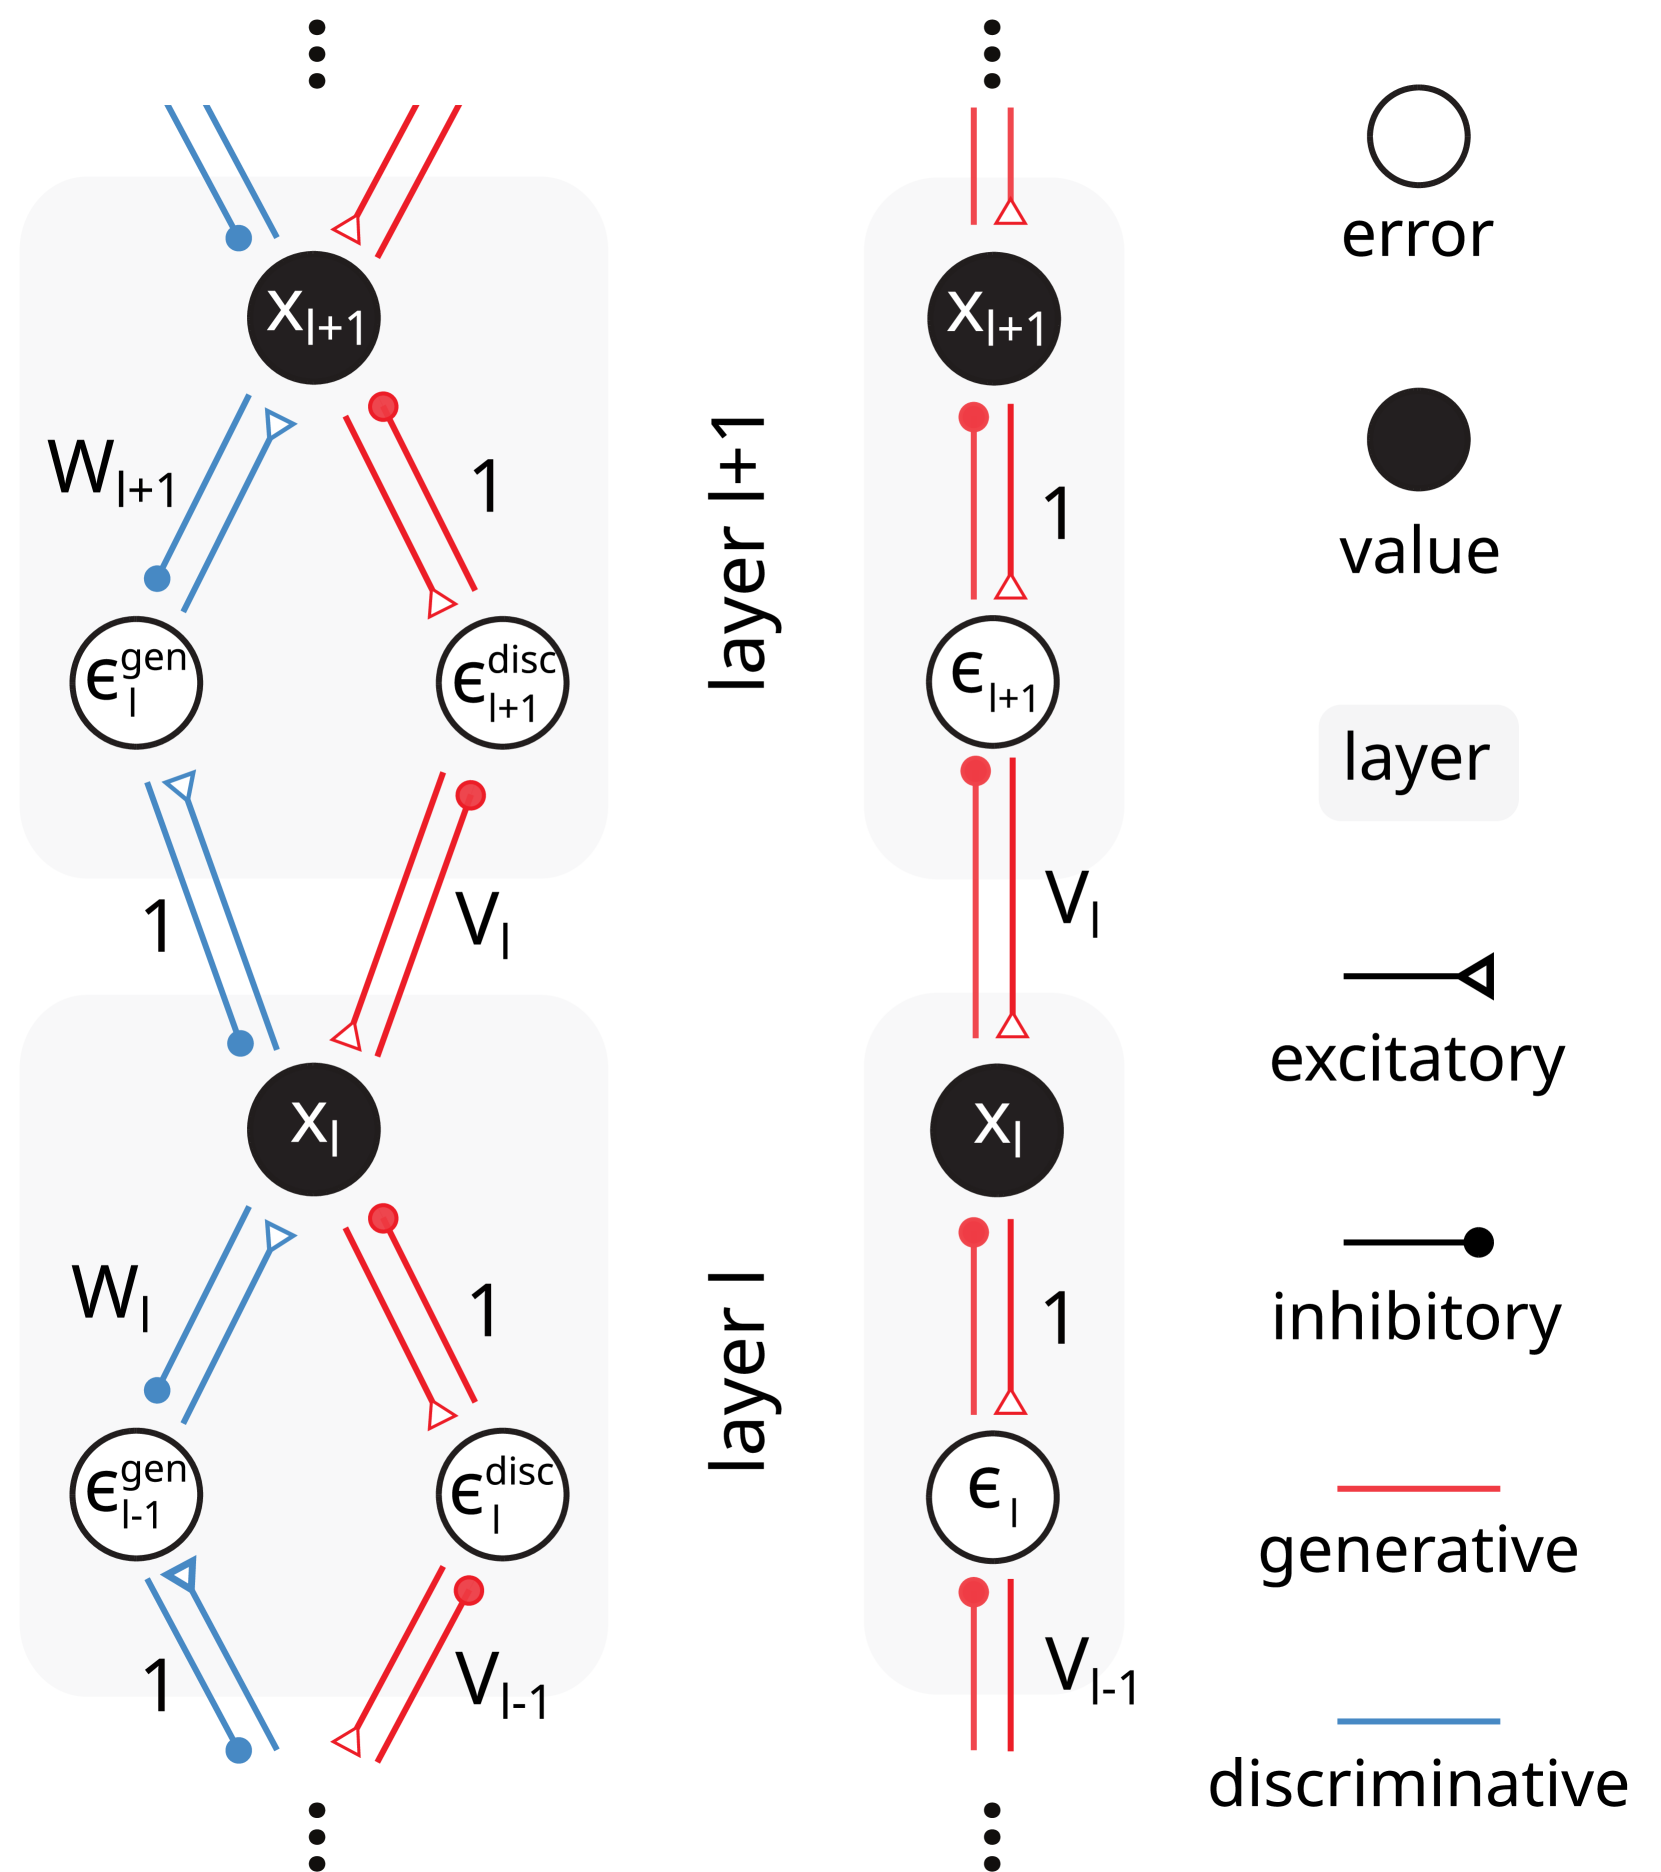
\includegraphics[scale=0.13]{x2.png}
   \caption{bPC(左)とdiscPC(右)の神経的実装}
   \label{neural_implementation}
\end{figure}
\subsubsection{柔軟な学習}
bPCは,教師あり学習と教師なし学習の両方で学習できる.いずれの場合も,中間層(層2から$L-1$)のニューロンは入力値に固定はされず,式5に示すニューラルダイナミクスに従って進化する.教師あり学習では,第1層$x_1$は入力値に固定され,最上層$x_L$はターゲットラベルに固定される.教師なし学習では,$x_L$は固定されず,bPCは入力の圧縮表現を学習する.$x_L$内のニューロンのサブセットのみがラベル情報に固定され,他のニューロンは固定されない混合学習も可能になる.この設定では,モデルはラベルを推論し,関連する圧縮表現を学習することができる.
\subsection{実験}
\subsubsection{教師あり分類と生成}
まず,単一のbPCモデルが識別タスクと生成タスクを同時に実行できることを示す.この実験では,bPCは画像とラベルの関連付けを学習し,入力画像を分類し,ラベルが与えられた場合にクラスの平均画像を生成できるようになる.2つの隠れ層 (各256ニューロン) を持つ同じアーキテクチャのMNISTおよびFashion-MNISTデータセットで,bPCをdiscPC,genPC,hybridPC,およびそれらのバックプロパゲーション同等のものと比較する.トレーニング中は,層$x_1$を画像に固定し,層\;$x_L=x_4$\;を対応するワンホットラベルに固定した (図\ref{ex_result1}A).トレーニング後,画像のみを与えられた状態で分類精度を測定することにより,識別性能を評価した.具体的には,層$x_1$を画像に固定し,100回の推論ステップ後に層$x_L$でラベルを推論した.生成性能は,各クラス ラベルから生成された画像と,そのクラスに対応する平均画像との間の二乗平均平方根誤差 (RMSE) によって評価した. $x_L$をクラスラベルに固定し,100ステップの反復推論を実行した後,$x_1$に生成画像を取得した.
\begin{figure}[htbp]
   \centering
   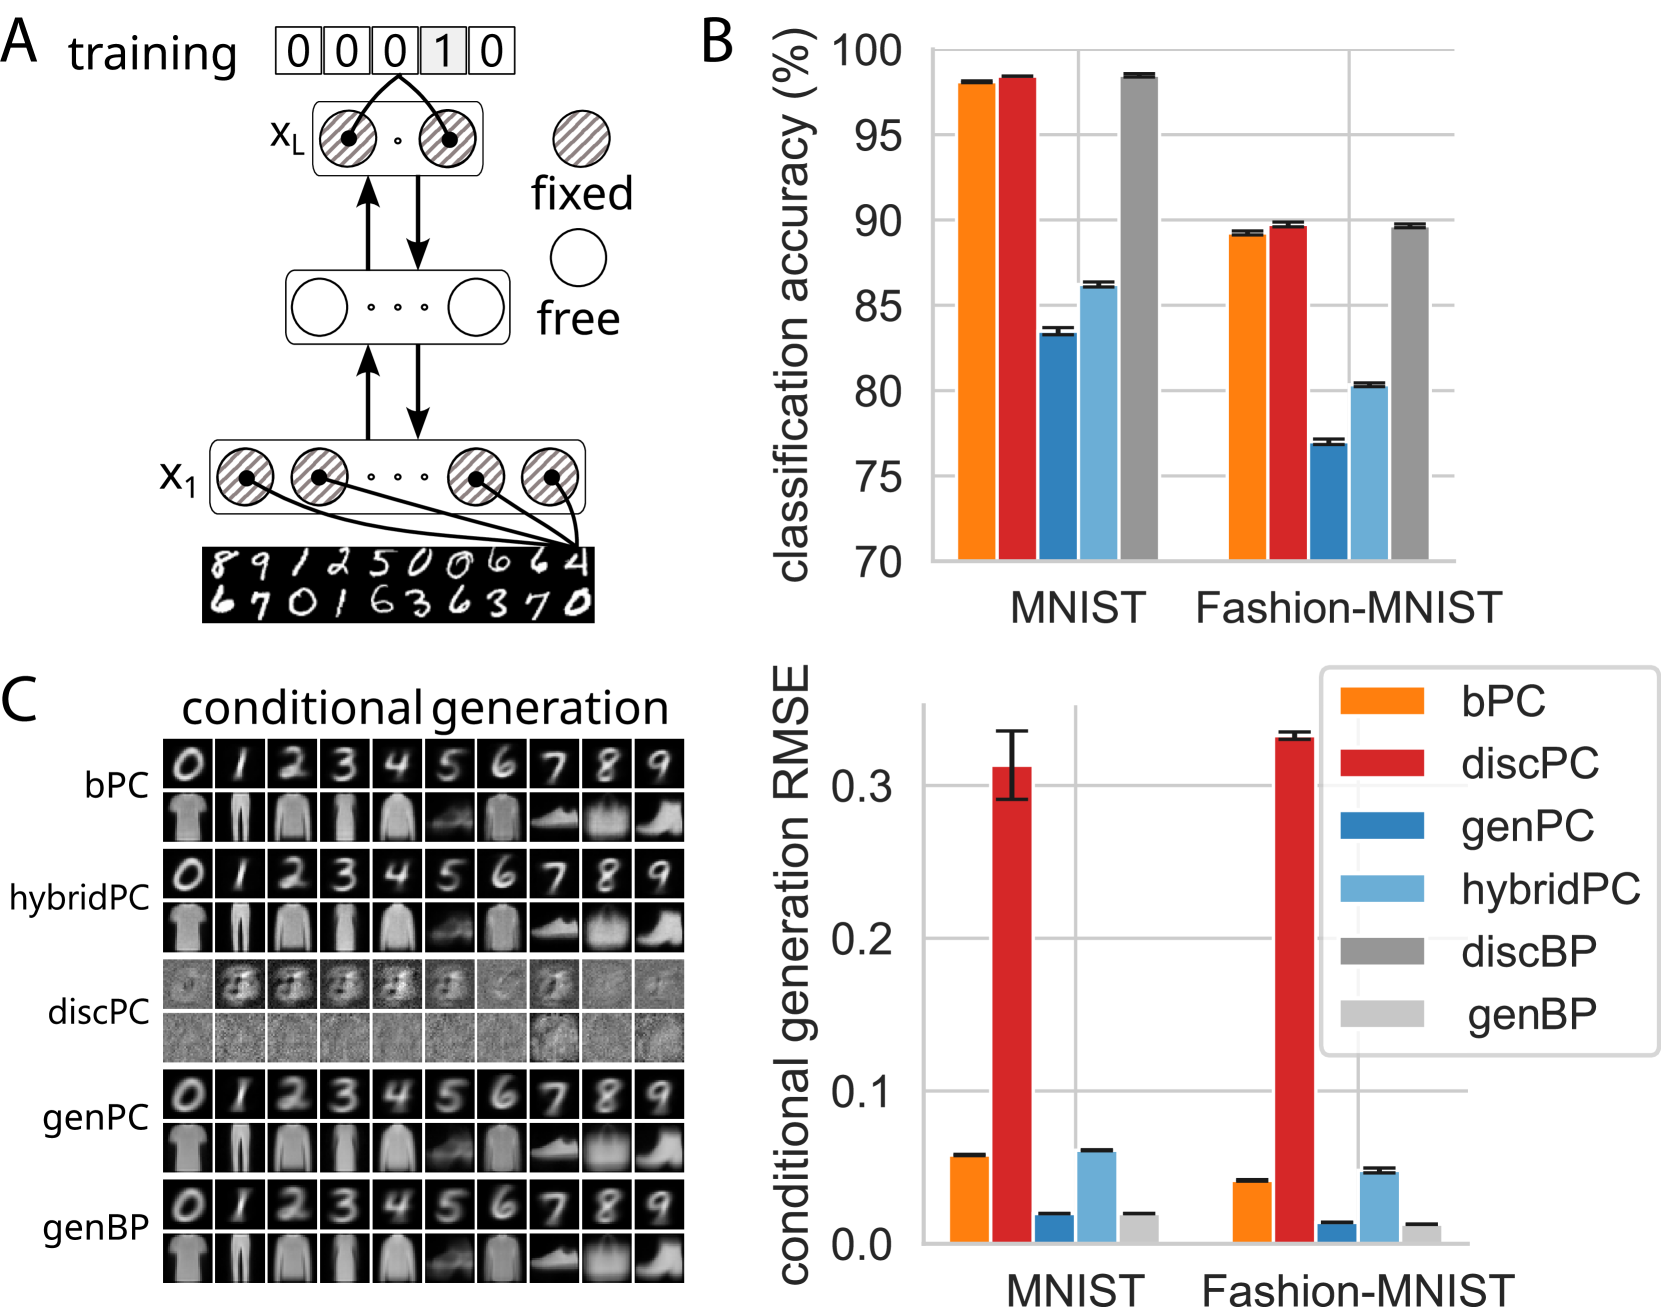
\includegraphics[scale=0.2]{x3.png}
   \caption{bPCは,MNISTとFashion-MNISTを正確に分類し,クラス平均画像を生成する.A:トレーニングセットアップ.モデルは,$x_1$を画像に固定し,$x_L$をラベルに固定してトレーニングされる.B:モデルの分類精度.C:クラスラベルを条件として生成された画像の例(左)と,生成された画像と各クラスの平均画像間のRMSE(右).}
   \label{ex_result1}
\end{figure} \\
図\ref{ex_result1}Bは,モデル間の分類精度と生成RMSEの比較を示している.bPCは,両データセットにおいて,discPCおよびdiscBPと同等の分類精度を達成している.一方,genBPとhybridPCは精度が低くなっている.生成性能に関しては,bPCはgenPC,hybridPC,genBPと同等のRMSEスコアを示しているが,discPCは生成エラーが著しく高くなっている.discPCから生成された画像には,クラスに関連する特徴がほとんど含まれていないが,bPCやその他のモデルは,各クラスについて明瞭で代表的な画像を生成する(図\ref{ex_result1}C).
\par
これらの結果は,単方向PCモデルがそれぞれの専門領域においてのみ優れているという,これまで報告された結果を裏付けるものである.discPCは学習最小値が一意ではないため生成に失敗し,genPCとhybridPCは分類精度が低い.対照的に,bPCは生成タスクと識別タスクを同時に実行する際に優れた性能を発揮する.注目すべきは,bPCは生成タスクと識別タスクの2つの経路を個別に維持するために必要なニューロンの半分しか使用しないため,エネルギー効率が向上する可能性があることである.
\par
また,トップダウン予測誤差の大きさが大きいため,識別重み付け$(\alpha_{disc})$を生成重み付けよりも高く設定する必要があることも判明した.
\subsubsection{教師無し表現学習}
次に,bPCが教師なしで圧縮表現を学習することを示す.MNIST,Fashion-MNIST,CIFAR-10,およびCIFAR-100データセットを使用して,bPC,genPC,hybridPC,およびそれらのBP同等物の表現学習パフォーマンスを,複雑さが増すタスク全体で評価した.discPCは,教師なし学習を実行できないため評価しなかった.レイヤー$x_1$のみが入力画像に固定され,他のすべてのレイヤーは任意になっているモデルをトレーニングした (図\ref{ex_result2}Aを参照).MNISTおよびFashion-MNISTモデルには,2つの隠し層 (それぞれ256ニューロン) と,30ニューロンの表現層$x_L$があった.
\begin{figure}[htbp]
   \centering
   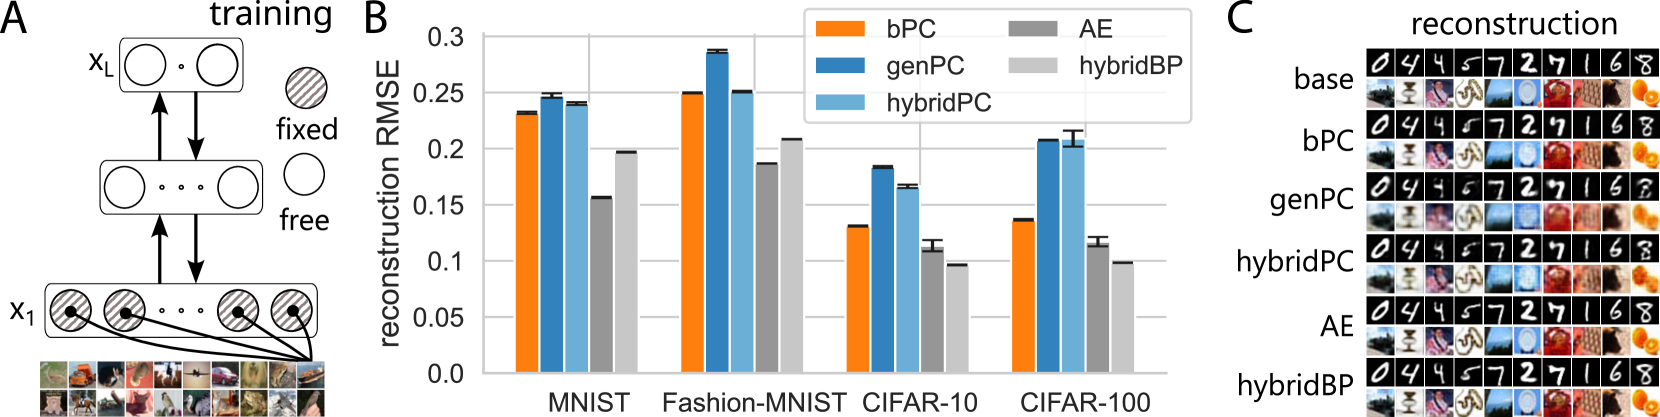
\includegraphics[scale=0.25]{x4.png}
   \caption{bPCは,低次元表現の学習において他のPCモデルよりも優れた性能を発揮.A:入力画像に$x_1$のみが固定されたトレーニングセットアップ.B:モデルとデータセット間の再構成RMSE.C:再構成の例.}
   \label{ex_result2}
\end{figure}
モデルの高速推論能力を評価するため,重み更新間の推論ステップ数を8に制限して学習を行った.CIFARモデルは5つの畳み込み層と256ニューロンからなる表現層で構成され,32ステップの推論で学習された.学習を安定化し,表現を制限するために,層$x_L$で活動減衰が用いられた.学習後,$x_1$の入力画像に対し100ステップの推論を行った後,$x_L$に表現が得られた.$x_L$をある表現に固定し,層$x_1$を$x_{L−1}$に再初期化した後,100ステップの推論で画像を再構成した.元の画像と,それらの表現から再構成された画像との間のRMSEを測定した.
\par
図\ref{ex_result2}Bは,bPCが一貫してgenPCよりも低いRMSEを達成し,性能が優れていることを示している.MNISTおよびFashion-MNISTでは,bPCはhybridPCの性能に匹敵する.CIFAR-10やCIFAR-100などのより複雑なデータセットでは,bPCはhybridPCを大幅に上回る.これらの場合,BPベースのモデルのパフォーマンスレベルに近づく.これらの結果は,各モデルの画像再構成のサンプルとともに,図\ref{ex_result2}Cにも示されている.bPCのgenPCに対する優れた表現学習能力は,bPCのボトムアップ経路によるフィードフォワード初期化が,初期の神経活動を最適状態に向けて微調整する高速な償却推論として機能することを示唆している.これは,推論ステップが限られている場合に特に役立つ.bPCがhybridPCよりも優れている理由は,反復推論中に潜在ニューロンに感覚情報を伝えるボトムアップの重み$V_l$が推論ダイナミクスに積極的に関与するためと考えられる.これは,CIFARデータセットのように感覚入力がより複雑な場合に特に重要になる.bPCにおける計算の局所的な性質は,学習効率は低くなるが,より妥当な実装につながるため,BPベースのモデルよりもわずかにパフォーマンスが劣る原因となっている可能性がある.
\subsubsection{教師あり学習と教師なし学習の組み合わせ}
ここでは,以前に説明した教師あり設定と教師なし設定を統合して,bPCが識別能力と圧縮表現を同時に開発できることを示す.MNIST,Fashion-MNIST,およびCIFAR-10データセットで,bPC,hybridPC,およびそれらのBPベースの同等物をトレーニングした.トレーニング中は,レイヤー$x_1$を入力画像に固定し,最上位レイヤー$x_L$をone-hotラベルに部分的に固定し,$x_L$の残りのニューロンは補完的な表現を学習できるようにした (図\ref{ex_result3}A を参照).前のセクションと一致して,MNISTモデルとFashion-MNISTモデルは,それぞれ256ニューロンの2つの隠し層で構成され,レイヤー$x_L$は40ニューロン (10 はラベル専用,30 は表現用) で構成されている.CIFAR-10モデルは,最大プーリングを備えた4つの隠れ畳み込み層と,266ニューロン (10 はラベル用,256 は表現用) を含む潜在層$x_L$を持つ畳み込みアーキテクチャを採用した.さらに,$x_L$の表現ニューロンには活動減衰が適用された.分類精度は画像のみ(セクション2.4.1と同様)を用いて測定され,生成品質は表現から画像を再構成することで評価された(セクション2.4.2と同様).重要な違いは,$x_L$を推論された表現と画像ラベルに固定することで画像を再構成する点である.
\par
図\ref{ex_result3}Bは,bPCがすべてのデータセットにおいてBPモデルと同等の分類精度を達成していることを示している.さらに,特にCIFAR-10において,bPCはハイブリッドPCを大幅に上回る.ハイブリッドPCは,bPCよりも45\%以上低い精度を示している.生成品質に関しては,図\ref{ex_result3}Dは,bPCがすべてのデータセットにおいてハイブリッドPCと同等の再構成誤差を達成していることを示している.
\begin{figure}[htbp]
   \centering
   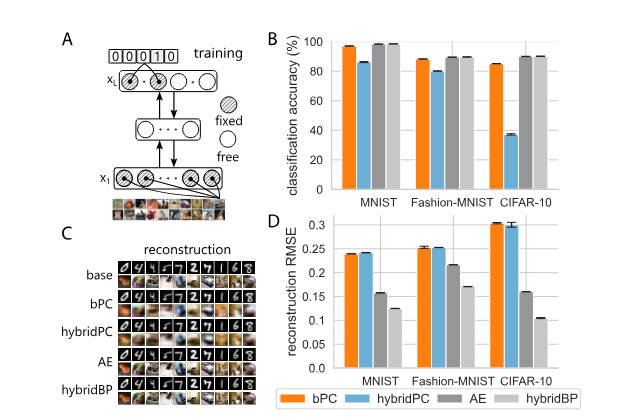
\includegraphics[scale=0.8]{x5.png}
   \caption{bPCは,画像の低次元表現を共同学習し,正確に分類できる唯一のPCモデル.A:潜在層がクラスラベルに部分的にのみクランプされているトレーニング設定.B:分類精度.C:MNISTおよびCIFAR10における再構成の例.D:再構成RMSE.}
   \label{ex_result3}
\end{figure} \\
図\ref{ex_result3}Cの再構成例は,bPCがクラス平均画像の生成にとどまらず,形状,色,空間位置(例えば,異なるスタイルで「4」を生成する)などの特徴を捉えていることを示している.しかし,識別ボトムアップ経路における最大プーリング操作によって導入されたアーティファクトのために,bPCのCIFAR-10再構成には細かい詳細が欠けており,これが生成トップダウン再構成プロセスに影響を与えている.
\par
その結果,bPCは,初期化に最大プーリングのみを使用するハイブリッドPCよりも,グリッド状のアーティファクトが顕著に現れ,生成層と識別層を別々に持つBPモデルよりも大幅にグリッド状のアーティファクトが顕著になる.最大プーリングを削除するとアーティファクトは除去されるものの,分類精度は低下する.しかしながら,最大プーリングを除外した場合でも,bPCの分類精度はハイブリッドPCを大幅に上回り,生成性能は同等のままで変わらない.
\subsubsection{共有された潜在層は偏りや過学習を防ぐ}
bPCが識別タスクと生成タスクの両方を同時にうまく実行できる理由を理解するために,そのエネルギーランドスケープ(式\eqref{bPC_Energy})を調べる.まず,エネルギーランドスケープを視覚化できる単純な2次元非線形分類問題であるXORタスクを検討する.bPCのエネルギーランドスケープを個々のgenPCおよびdiscPCによって開発されたものと比較し,独立した潜在層ではなく共有された潜在層の利点を調査する.$x_1$を2次元入力に,$x_4$をスカラー出力に固定して,それぞれ16ニューロンの2つの隠し層を持つbPC(図\ref{ex_result4}A 下部),genPC,および discPC (図\ref{ex_result4}A 上部) をトレーニングした.このセットアップでは,bPC のパラメーター数は genPC と discPC を合わせた数と同じになるが,ニューロン数は半分である.トレーニング後のエネルギー ランドスケープを図\ref{ex_result4}6B に示す.一方,genPCは各クラスの平均においてエネルギー最小値を生成するため,XORデータの真の構造を捉えることができない.特に,discPCとgenPCを別々の目的を持つ単一のモデルに統合した場合,結果として得られるエネルギーランドスケープには,最小値が広く偏っているという両方の問題が残ってしまう.一方,bPCはデータポイントの周囲に,明確で局所的な最小値を学習できる.
\begin{figure}[htbp]
   \centering
   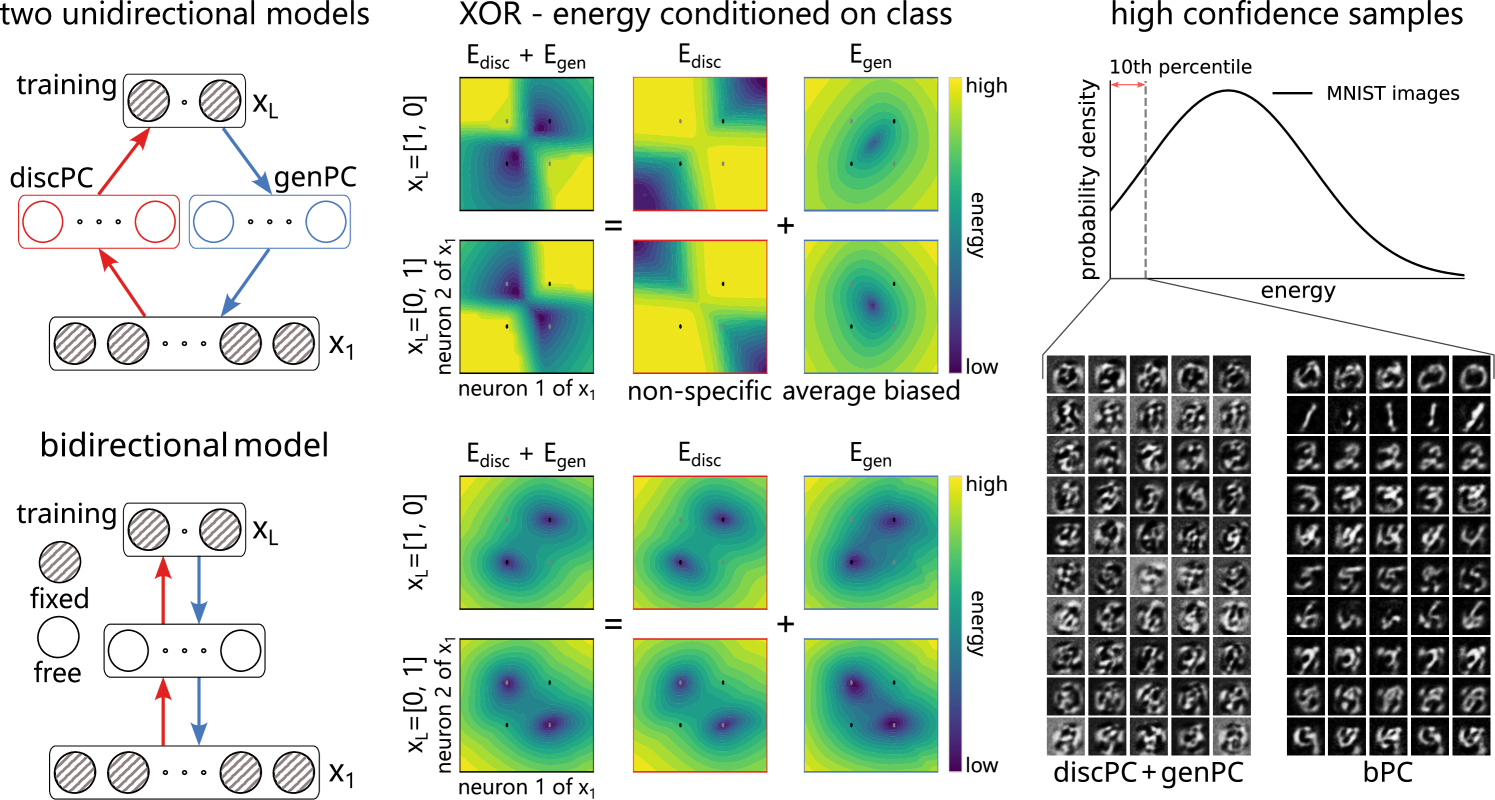
\includegraphics[scale=0.26]{x6.png}
   \caption{bPCは,生成と分類の両方に適したエネルギーランドスケープを構築.A:bPC(下)と,discPCとGenPCを個別に学習させた場合(上)を比較する.B:XOR学習後のモデルのエネルギーランドスケープの可視化.識別エネルギー,生成エネルギー,および合計エネルギーが表示されている.C:モデルによって高い確率(下位10\%のエネルギー)と判断されたMNISTサンプル.}
   \label{ex_result4}
\end{figure}
\par
次に,セクション2.4.1で検討したモデルのMNISTサンプル生成能力を評価することにより,これらの観察の一般化可能性を検証した.具体的には,最上位層$x_L$を特定の数字ラベルに固定し,入力層$x_1$をランダムに初期化し,モデルがMNISTテスト画像で観測された平衡エネルギーの最低10\%以下のエネルギー値に達するまで推論の更新を実行した.discPC-genPCの組み合わせモデルの場合,生成されたサンプルが両方のコンポーネントでこの低エネルギー基準を満たすことを要求した.この設定はサンプリングプロセスとして機能し,モデルによって可能性が高いと見なされた画像を検査することができる.図\ref{ex_result4}Cは,bPCによって生成されたサンプルが,過度の背景ノイズと定義の曖昧な数字の形状を含むことが多い,discPC-genPCの組み合わせモデルのサンプルよりも大幅に現実的であることを示している.サンプルの品質を定量化するために,生成された数字が分類器によってどれだけ簡単にラベル付けできるかを評価するインセプションスコアと,画像の品質と多様性を測定するフレシェインセプション距離(FID)を使用した.bPCは複合モデルを大幅に上回り,インセプションスコア(bPC:6.05±0.17 vs. 複合:3.62±0.03,5シードの平均値±標準誤差)が高く,FIDスコア(bPC:44.4±2.2 vs. 複合:140.5±2.1)が低くなった.BPベースの複合モデル(discBP + genBP)との比較を繰り返したが,やはりbPCの方がより高品質なサンプルを生成した.
\par
これらの結果は,セクション 2.
2.4.1 の観察に対する詳細なメカニズムの説明を提供する. discPC は,幅広いエネルギー最小値を持つ無意味な OOD 画像に自信を持って低エネルギーを割り当てるため,画像生成のパフォーマンスが低下している. genPC は各クラスの平均画像のみを低エネルギーとして認識するため,新しいパターンは平均クラスの画像までの距離に基づいて分類されるテンプレート マッチング メカニズムに依存する. 一方,bPC は,これら 2 つのエネルギー関数 ($E_{disc}$ と $E_{gen}$) が共同で最小化され,お互いに相互正規化として機能するため,より選択的なエネルギー ランドスケープを開発できる. これは,図\ref{ex_result4}B の下のパネルから確認することができる.bPC の $E_{gen}$ は,個々のデータ ポイントも含むように $E_{disc}$ によって引き延ばされるが,$E_{disc}$ は,より小さく,より専用の最小値を持つように $E_{gen}$ によって圧縮される.
\subsubsection{生物学的に関連する課題における学習}
まず,脳が連想を形成する典型的な方法であるマルチモーダル学習における bPC を調査する.教師あり学習タスクをシミュレートする場合,ラベルの情報は通常,単純化のために最上位層に提供されるが,人間が情報を取得するときには,カテゴリは別のモダリティで表現されることがよくある.たとえば,子供が動物の名前を覚えるとき,これらの名前は親によって話され,聴覚皮質を介して処理される (図\ref{ex_result5}A).マルチモーダル機能を評価するため,MNIST データセットと Fashion-MNIST データセットを使用して,バイモーダルタスクで bPC と genPC を比較した.1 つの潜在層が 2 つの別々の入力層に接続され (図\ref{ex_result5}A),1 つはラベルの one-hot ベクトルに固定され,もう 1 つは対応する入力画像に固定された階層モデルをトレーニングした.bPC モデルには,各入力層と潜在層の間のボトムアップとトップダウンの予測が含まれていたが,genPC は潜在層から入力層へのトップダウンの予測のみを組み込んでいた.
\par
トレーニング後,分類精度と平均画像再構成誤差を測定することで,クロスモーダル情報伝達を評価した. 1 つのモダリティに入力を与え,反復推論を実行した. 次に,入力なしのモダリティの活動を,正しいラベルまたはクラス平均画像と比較した. 図\ref{ex_result5}B,C,および D は,バイモーダル bPC モデルが,分類精度と画像再構成性能の両方で genPC を大幅に上回っていることを示している. バイモーダル bPC は,ボトムアップとトップダウンの対称性により,セクション 4.1 で紹介した bPC モデルと同等であり,両方のタスクで成功することが証明されているため,この結果は予想通りである. 言い換えれば,bPC の隠れ層は自然に連合皮質領域をモデル化している. 一方,genPC は,1 つの経路が画像を予測し (genPC と同様),もう 1 つがラベルを予測する (discPC と同様) マルチモーダル連合皮質をモデル化するために意図的に再構成する必要がある. その結果,バイモーダル genPC は両方のモデルタイプの制限を継承し,分類と生成の質が低下する.
\begin{figure}[htbp]
   \centering
   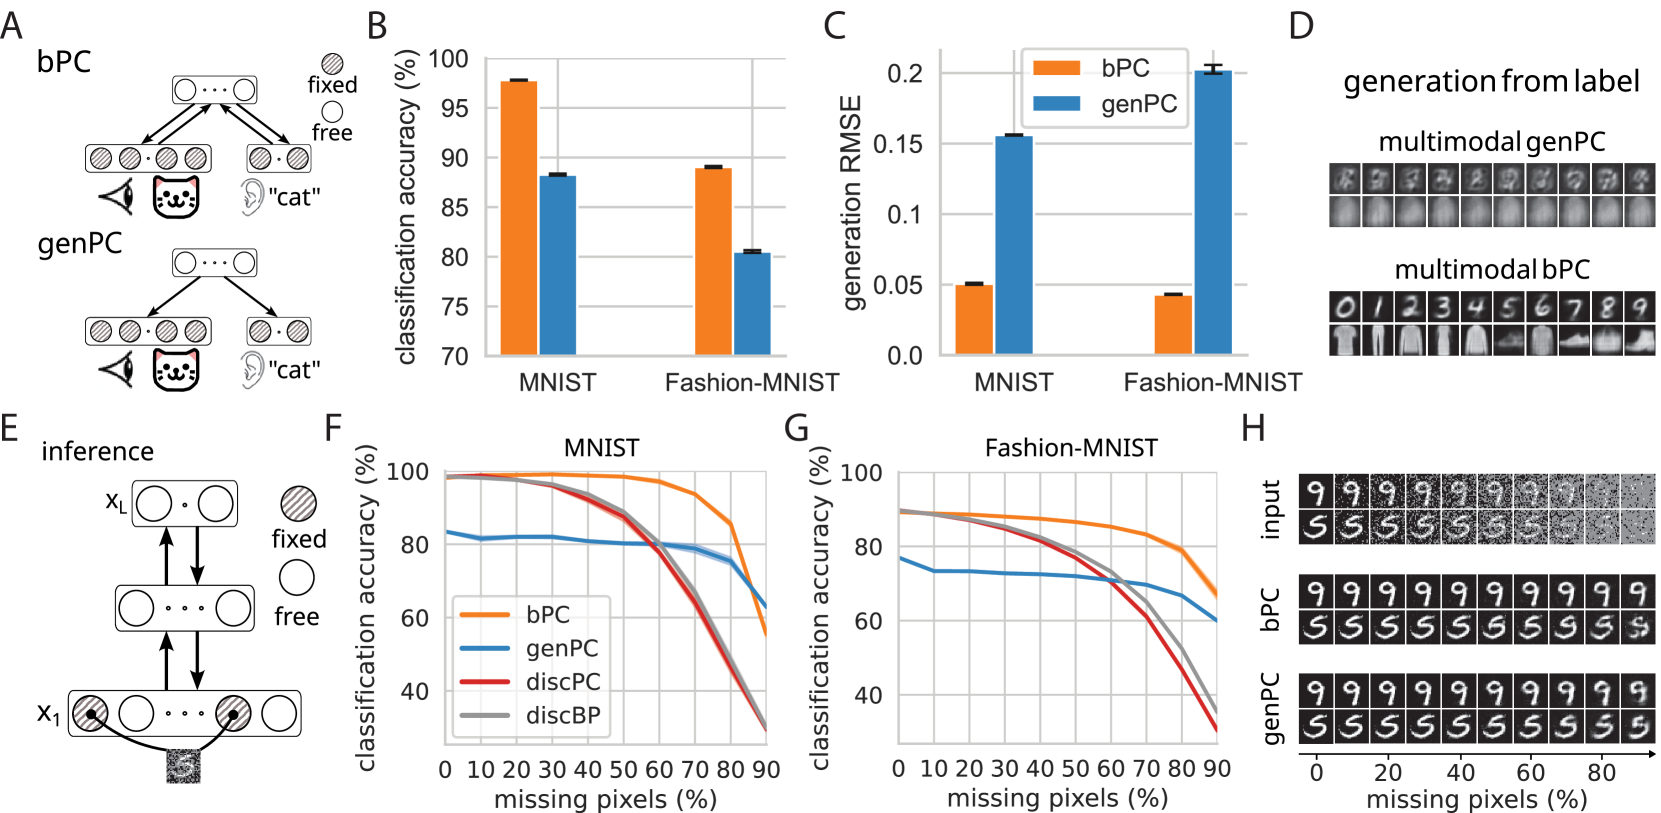
\includegraphics[scale=0.23]{x7.png}
   \caption{マルチモーダル学習におけるbPCの性能と欠損情報に対する堅牢性.A:バイモーダルbPCとgenPC.バイモーダルbPCはセクション2.4.1のユニモーダルbPCと完全に同等であることに注意する必要がある.ここでは視覚的な目的のために簡略化されています.B:バイモーダルPCモデルの分類精度.CとD:生成RMSEと例.E:部分的に遮蔽された感覚入力に対するモデル評価.FとG:それぞれMNISTとFashion-MNISTにおける欠損ピクセルの割合に対する分類精度.H:genPCとbPCの推論後のx1のアクティビティ.}
   \label{ex_result5}
\end{figure}
次に,脳は不完全または遮蔽された視覚シーンであっても,分類などの重要な認知機能を保持することが知られているため,部分的に欠損した情報に対する bPC の堅牢性をテストする.セクション 2.4.1 のトレーニング済みモデル (bPC,genPC,discPC,discBP) を使用して,MNIST および Fashion-MNIST で欠損ピクセルのレベルを増加させた場合 (0\% から 90\%) の分類精度を評価した.$x_1$ の観測ニューロンの活動を観測ピクセルに固定し,観測されていないニューロンは空けておき,図\ref{ex_result5}E に示すように活動ゼロに初期化する.欠損データによる推論収束が遅いことに対応するため,評価前に推論期間を延長した.
\par
図\ref{ex_result5}F および G に示すように,bPC は最大 80\% のピクセルが欠落していても高い分類精度を維持する.genPC も妥当なパフォーマンスを維持するが,全体的な精度はオクルージョンのレベル全体で bPC よりも低くなる.対照的に,discPC と discBP は,欠落入力が 50\% を超えるとパフォーマンスが急激に低下する.bPC の堅牢性は,トップダウン予測に由来している.つまり,推論によって欠落入力を積極的に埋め,トップダウンの生成事前確率とボトムアップの証拠を統合して入力を再構築する.図\ref{ex_result5}H は,欠落入力が bPC によって埋められた入力画像の例を示している.genPC にもこの能力はあるものの,識別力が弱いという欠点がある.対照的に,discPC と discBP はトップダウン生成メカニズムがないため,欠落情報を推論できない.
\subsection{結論}
視覚処理に関する経験的および理論的洞察に基づき,我々は双方向予測符号化を提案する.これは,生成処理と識別処理を統合した,生物学的に妥当な視覚推論の計算モデルである.我々は,bPCが教師あり分類学習タスクと教師なし表現学習タスクの両方で効果的に機能し,従来の予測符号化モデルを一貫して上回るか同等の性能を発揮することを実証した.実験により,bPCの性能は,識別タスクと生成タスクの両方に同時に最適化されたエネルギーランドスケープを開発する能力から生まれ,それによって分布外データに対する堅牢性が向上することが明らかになった.さらに,マルチモーダル統合や部分的に欠損した入力を伴う推論など,生物学的に関連するシナリオにおけるbPCの有効性を示した.全体として,bPCは,脳内で柔軟な推論がどのように発現するかについての仮説を提示するとともに,機械学習アプリケーションにおける識別モデルの堅牢性を高める方法も提供する.

\end{document}